\section{Kilka słów o~zasadach typografii}

\noindent Proszę o~używanie następujących zasad:
{\raggedright
\begin{itemize}
\item nie zostawiać na końcu wiersza tzw. ,,wiszących spójników''
  (np. w, z...)
\item pisać \verb|\dywiz| w~miejsce -, czyli np.
  \verb|biało\dywiz czerwony| zamiast \verb|biało-czerwony|, ale
  \verb|$n$-wymiarowy|, a~nie \verb|$n$\dywiz wymiarowy|
\item pisać \verb|\polishendash| w~miejsce --, czyli
  np. \verb|twierdzenie Bolzano\polishendash Weierstrassa| a~nie
  \verb|twierdzenie Bolzano--Weierstrassa|
\item pisać półpauzę \verb|\ppauza|, czyli na przykład
  \verb|jak wspomnieliśmy\ppauza dowód jest poprawny|
\item pierwszy wiersz akapitu następujący po rozdziale lub punkcie bez
  wcięcia akapitowego (czyli \verb|\noindent|)
\end{itemize}\par}


\section{Zasada maksimum i~jej zastosowanie do badania szeregów
  potęgowych}

\noindent Celem tego rozdziału jest prezentacja zasady maksimum oraz
zastosowanie jej do badania szeregów potęgowych.

\subsection{Zasada maksimum}

\noindent Dowód poniższego twierdzenia można znaleźć na przykład
w~książce \cite{complex}.
\begin{theorem}[Zasada maksimum]\label{tw-1}
  Niech $\mathbb{D}$ będzie obszarem na płaszczyznie zespolonej.
  Jeśli $f\in H(\mathbb{D})$ oraz istnieje taki punkt
  $z_0\in\mathbb{D}$, że
  \[
  \sup \bigl\{|f(z)| : z\in\mathbb{D}\bigr\} =|f(z_0)|,
  \]
  to funkcja $f$ jest stała w~zbiorze $\mathbb{D}$.
\end{theorem}

\begin{proof}
\lipsum[1-4]
\end{proof}

\begin{definicja}
  Funcją całkowitą nazywamy finkcję mającą pochodną w~każdym punkcie
  płaszczyzny zespolonej.
\end{definicja}

\subsection{Suma szeregu geometrycznego}

\noindent Podstawową rolę w~dalszych rozważaniach odgrywać będzie
poniższe twierdzenie.

\begin{theorem}\label{tw-2}
  Jeśli $|x|<1$, to
  \begin{equation*}
    \sum_{n=0}^\infty x^n=\frac{1}{1-x}.
  \end{equation*}
\end{theorem}

\begin{proof}
  Ze wzoru na sumę skończonej ilości wyrazów ciągu geometrycznego
  wynika, że
  \begin{equation}\label{w-1}
    \sum_{k=0}^n x^k=\frac{1-x^{n+1}}{1-x}.
  \end{equation}
  Zauważmy teraz, że jeśli $|x|<1$, to granica wyrażenia stojącego po
  prawej stronie znaku równości we wzorze \eqref{w-1} istnieje oraz
  \[
  \lim_{n\to\infty} \sum_{k=0}^n x^k=\lim_{n\to\infty}
  \frac{1-x^{n+1}}{1-x} =\frac{1}{1-x}.
  \]
\end{proof}

Z~twierdzenia \ref{tw-2} otrzymać można (w~miejsce $x$ podstawiając
$-x$) poniższą równość.

\begin{wniosek}
Jeśli $|x|<1$, to 
\begin{equation}\label{w-2}
\sum_{n=0}^\infty (-1)^n x^n=\frac{1}{1+x}.
\end{equation}
\end{wniosek}

\lipsum[1-5]

\begin{uwaga}
  Podstawmy w~równościach \ref{w-1} oraz \ref{w-2} w~miejsce $x$
  wyrażenie $x^2$.  Poniżej prezentujemy otrzymane wykresy funkcji.

\begin{figure} 
  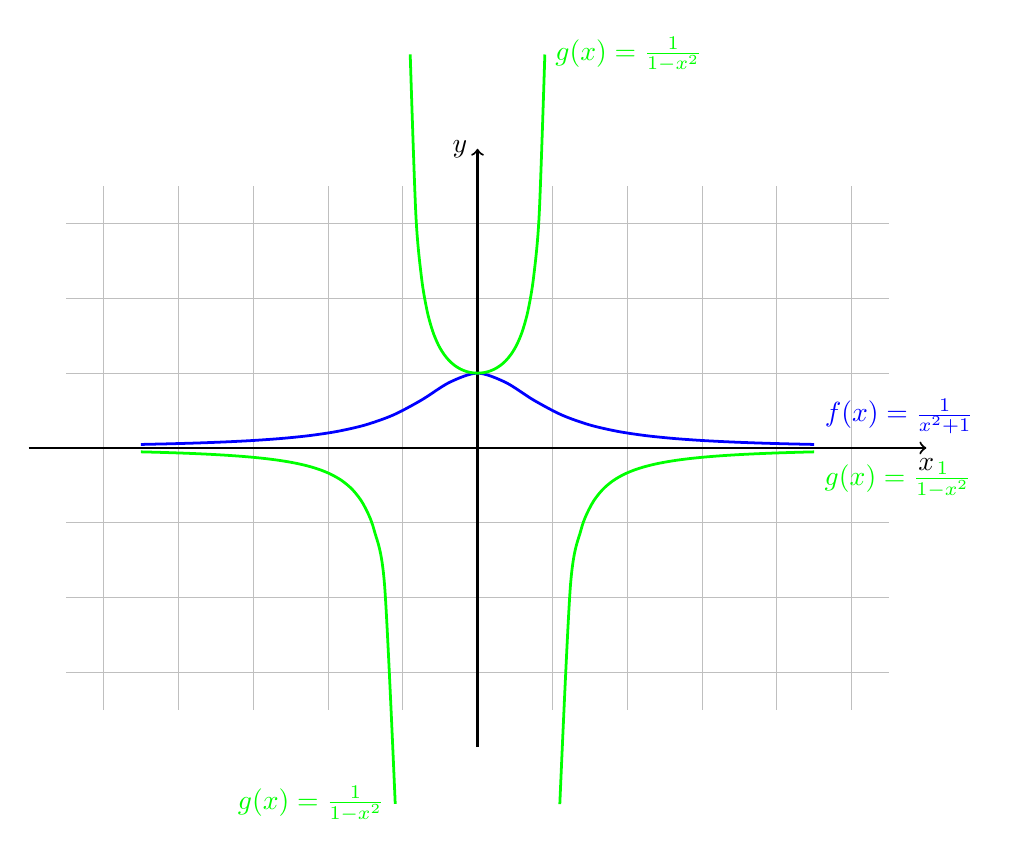
\begin{tikzpicture}[scale=.95]
\draw[step=1,lightgray,very thin] (-5.5,-3.5) grid (5.5,3.5);
\draw[line width=.75pt,->] (-6,0) -- (6,0) node[below] {$x$};
\draw[line width=.75pt,->] (0,-4) -- (0,4) node[left] {$y$};
%
\draw[line width=1pt,blue,variable=\x,smooth,domain=-4.5:4.5]
plot({\x},{1/(\x*\x+1)}) node[above right] {$f(x)=\frac{1}{x^2+1}$};
%
\draw[line width=1pt,green,variable=\x,smooth,domain=-4.5:-1.1]
plot({\x},{1/(1-\x*\x)}) node[left] {$g(x)=\frac{1}{1-x^2}$};
\draw[line width=1pt,green,variable=\x,smooth,domain=-.9:.9]
plot({\x},{1/(1-\x*\x)}) node[right] {$g(x)=\frac{1}{1-x^2}$};
\draw[line width=1pt,green,variable=\x,smooth,domain=1.1:4.5]
plot({\x},{1/(1-\x*\x)}) node[below right] {$g(x)=\frac{1}{1-x^2}$};
\end{tikzpicture}
\caption{Wykresy funkcji $f(x)=\frac{1}{x^2+1}$ (kolorem niebieskim)
  oraz $g(x)=\frac{1}{1-x^2}$ kolorem zielonym}
\end{figure}
\end{uwaga}

\section{Jak wykonywać rysunki w~programie \LaTeX?}

\noindent Celem tego rozdziału jest prezentacja sposobu przygotowania rysunków
z~wykorzystaniem pakietu \emph{tikz} w~programie \LaTeX.

\subsection{Proste rysunki}

\begin{center}
\begin{tikzpicture}
\draw (0,0) circle (3);
\draw (0,0) -- (3,3);
\draw (0,0) -- (3.5,0);
\draw[line width=.75pt] (1,0) arc (0:45:1);
\node[above] at (.5,0) {$\alpha$};
\end{tikzpicture}
\end{center}

\lipsum[1]

\subsection{Wykresy funkcji}

\noindent Można również rysować wykresy funkcji.

\noindent 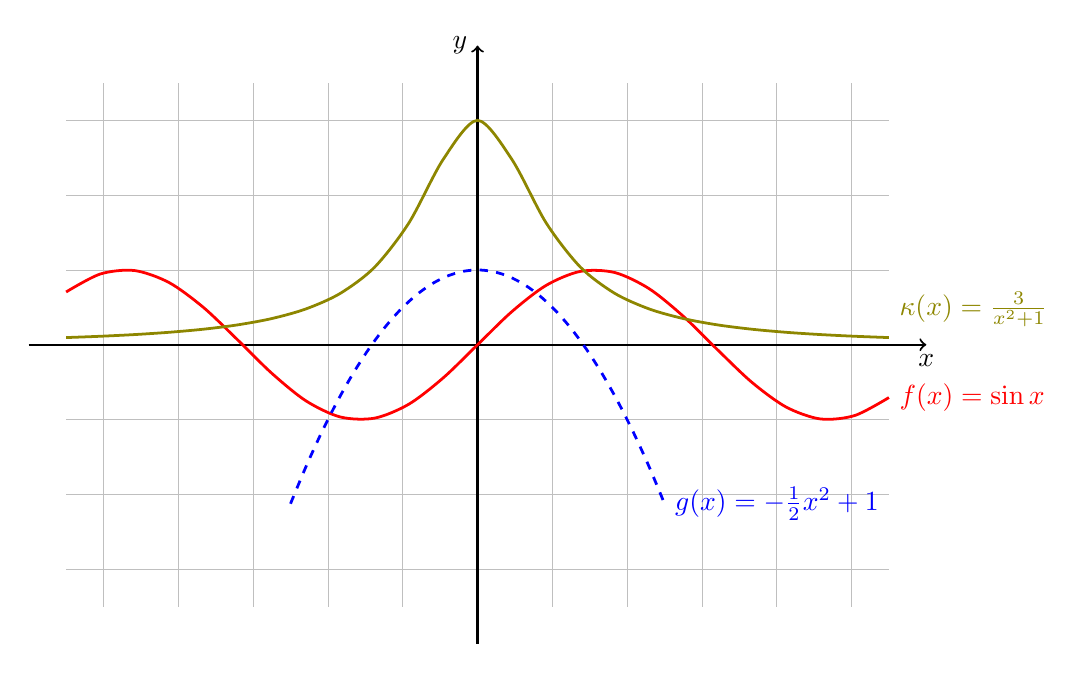
\begin{tikzpicture}[scale=.95]
\draw[step=1,lightgray,very thin] (-5.5,-3.5) grid (5.5,3.5);
\draw[line width=.75pt,->] (-6,0) -- (6,0) node[below] {$x$};
\draw[line width=.75pt,->] (0,-4) -- (0,4) node[left] {$y$};
\draw[line width=1pt,red,variable=\x,smooth,domain=-5.5:5.5]
plot({\x},{sin(\x r)}) node[right] {$f(x)=\sin x$};
\draw[line width=1pt,blue,dashed,variable=\x,smooth,domain=-2.5:2.5]
plot({\x},{-.5*\x*\x+1}) node[right] {$g(x)=-\frac{1}{2}x^2+1$};
\draw[line width=1pt,olive,variable=\x,smooth,domain=-5.5:5.5]
plot({\x},{3/(\x*\x+1)}) node[above right]
{$\kappa(x)=\frac{3}{x^2+1}$};
\end{tikzpicture}

\lipsum[1-6]